%%%%%%%%%%%%%%%%%%%%%%%%%%%%%%%%%%%%%%%%%%%%%%%%%%%%
% LECTURE 10
%%%%%%%%%%%%%%%%%%%%%%%%%%%%%%%%%%%%%%%%%%%%%%%%%%%%
% \section*{Review of Conduction}
% \addcontentsline{toc}{section}{Review of Conduction}
% %%%%%%%%%%%%%%%%%%%%%%%%%%%%%%%%%%%%%%%%%%%%%%%%%%%%
% \subsection*{Fundamental Laws of Conduction}
% \addcontentsline{toc}{subsection}{Fundamental Laws of Conduction}
% %%%%%%%%%%%%%%%%%%%%%%%%%%%%%%%%%%%%%%%%%%%%%%%%%%%%
% Two fundamental laws govern heat conduction problems:

% \begin{enumerate}
%     \item \textbf{Energy Balance (Conservation Law)}: Energy must be conserved over a domain
%     \[
%         \text{Energy}_\text{in} - \text{Energy}_\text{out} + \text{Energy}_\text{generated} = \text{Energy}_\text{stored}
%     \]
    
%     \item \textbf{Fourier's Law (Rate Law)}: Describes heat flow direction and magnitude at a point based on temperature gradient
%     \[
%         \vec{q} = -k \nabla T
%     \]
% \end{enumerate}

% The energy balance law describes the integrated result over a domain, while Fourier's law describes the point-wise behavior. When both laws are satisfied throughout the system, a unique solution exists.
% %%%%%%%%%%%%%%%%%%%%%%%%%%%%%%%%%%%%%%%%%%%%%%%%%%%%
% \subsection*{Control Volume Approach}
% \addcontentsline{toc}{subsection}{Control Volume Approach}
% %%%%%%%%%%%%%%%%%%%%%%%%%%%%%%%%%%%%%%%%%%%%%%%%%%%%
% A common source of confusion is the sign convention when applying energy balance:

% \begin{itemize}
%     \item When defining energy flux through a boundary, the direction of the normal vector determines whether energy is entering or leaving
%     \item If the heat flux vector $\vec{q}$ is aligned with the inward normal $\vec{n}$, it represents energy entering the system
%     \item Mathematically: $E_\text{in} = \int_A \vec{q} \cdot \vec{n} \, dA$, where $\vec{n}$ is the inward normal
% \end{itemize}

% Alternatively, one can define all energy as "in" and let the dot product determine the sign:
% \[
%     E_\text{in} = \int_A \vec{q} \cdot \vec{n}_\text{in} \, dA
% \]

% For simple problems with known heat flow directions:
% \begin{itemize}
%     \item Define energy explicitly as "in" or "out" based on flow direction
%     \item Use absolute values to avoid sign confusion
%     \item Energy generated is always a volumetric integral: $\int_V q''' \, dV$
%     \item Energy stored is $\rho c_p V \frac{\partial T}{\partial t}$
% \end{itemize}
% %%%%%%%%%%%%%%%%%%%%%%%%%%%%%%%%%%%%%%%%%%%%%%%%%%%%
% \subsection*{Common Misconceptions about Advection}
% \addcontentsline{toc}{subsection}{Common Misconceptions about Advection}
% %%%%%%%%%%%%%%%%%%%%%%%%%%%%%%%%%%%%%%%%%%%%%%%%%%%%
% Advection represents thermal energy transported by fluid motion, regardless of temperature:
% \begin{itemize}
%     \item Even a cold fluid (e.g., liquid nitrogen) brings thermal energy into a system
%     \item Advection is always $\rho c_p \vec{u} T$, where $T$ is absolute temperature
%     \item The sign of advection depends on flow direction, not whether the fluid is "hot" or "cold"
% \end{itemize}
% %%%%%%%%%%%%%%%%%%%%%%%%%%%%%%%%%%%%%%%%%%%%%%%%%%%%
% \subsection*{Special Heat Transfer Problems}
% \addcontentsline{toc}{subsection}{Special Heat Transfer Problems}
% %%%%%%%%%%%%%%%%%%%%%%%%%%%%%%%%%%%%%%%%%%%%%%%%%%%%
% \subsubsection*{Fin Equation}
% \addcontentsline{toc}{subsubsection}{Fin Equation}
% %%%%%%%%%%%%%%%%%%%%%%%%%%%%%%%%%%%%%%%%%%%%%%%%%%%%
% \begin{itemize}
%     \item Derived by approximating a 2D problem as 1D
%     \item Neglects temperature variation across the fin thickness
%     \item Assumes conduction along the fin with convection from the sides
%     \item Energy balance with this approximation yields the fin equation
% \end{itemize}
% %%%%%%%%%%%%%%%%%%%%%%%%%%%%%%%%%%%%%%%%%%%%%%%%%%%%
% \subsubsection*{Lumped Capacitance Method}
% \addcontentsline{toc}{subsubsection}{Lumped Capacitance Method}
% %%%%%%%%%%%%%%%%%%%%%%%%%%%%%%%%%%%%%%%%%%%%%%%%%%%%
% \begin{itemize}
%     \item Assumes uniform temperature throughout the solid
%     \item Contrary to intuition, this assumes conduction is very strong (not negligible)
%     \item Conduction within the material is much faster than heat transfer to the environment
%     \item Applicable when Biot number is small: $\text{Bi} = \frac{hL}{k} < 0.1$
% \end{itemize}
% %%%%%%%%%%%%%%%%%%%%%%%%%%%%%%%%%%%%%%%%%%%%%%%%%%%%
% \subsubsection*{2D Conduction and Separation of Variables}
% \addcontentsline{toc}{subsubsection}{2D Conduction and Separation of Variables}
% %%%%%%%%%%%%%%%%%%%%%%%%%%%%%%%%%%%%%%%%%%%%%%%%%%%%
% \begin{itemize}
%     \item Useful for solving problems with complex boundary conditions
%     \item Based on superposition principle
%     \item Decomposes arbitrary boundary conditions into simpler components (e.g., Fourier series)
%     \item Each component has a known analytical solution
%     \item Components are summed to obtain the complete solution
% \end{itemize}
% %%%%%%%%%%%%%%%%%%%%%%%%%%%%%%%%%%%%%%%%%%%%%%%%%%%%
% \subsubsection*{Numerical Methods for Conduction}
% \addcontentsline{toc}{subsubsection}{Numerical Methods for Conduction}
% %%%%%%%%%%%%%%%%%%%%%%%%%%%%%%%%%%%%%%%%%%%%%%%%%%%%
% Three main approaches:
% \begin{enumerate}
%     \item \textbf{Finite Difference Method}
%     \begin{itemize}
%         \item Assumes smooth, second-order solution
%         \item Approximates derivatives using nodal values
%         \item Good for regular geometries
%     \end{itemize}
    
%     \item \textbf{Finite Element Method}
%     \begin{itemize}
%         \item Uses shape functions between nodes
%         \item Value at any point depends only on immediate neighboring nodes
%         \item Minimizes overall error based on chosen shape functions
%         \item Better for irregular geometries
%     \end{itemize}
    
%     \item \textbf{Finite Volume Method}
%     \begin{itemize}
%         \item Guarantees energy conservation
%         \item Approximates heat flux between control volumes
%         \item Commonly used in heat transfer and fluid flow problems
%         \item Energy conservation is perfectly satisfied, though temperature field may have errors
%     \end{itemize}
% \end{enumerate}
%%%%%%%%%%%%%%%%%%%%%%%%%%%%%%%%%%%%%%%%%%%%%%%%%%%%
\section*{Introduction to Convection}
\addcontentsline{toc}{section}{Introduction to Convection}
%%%%%%%%%%%%%%%%%%%%%%%%%%%%%%%%%%%%%%%%%%%%%%%%%%%%
\subsection*{Fundamentals of Convection}
\addcontentsline{toc}{subsection}{Fundamentals of Convection}
%%%%%%%%%%%%%%%%%%%%%%%%%%%%%%%%%%%%%%%%%%%%%%%%%%%%
Convection is diffusion with motion can be conceptualized as:
\[
    \text{Convection} = \text{Diffusion} + \text{[Fluid] Motion}
\]

\begin{itemize}
    \item Convection is diffusion with motion, whether due to fluid flow or mass movement.
    \item Conduction is \textbf{only diffusion}, while convection involves both diffusion and advection (mass transport).
    \item If a material is moving (as dictated by your coordinate system), it should be treated as a convection problem, not a conduction problem.
    \item This course shifts focus from applying empirical correlations (as in undergraduate studies) to understanding the \textbf{mechanisms} behind them, formulating mathematical models, and generating new correlations.
    \item The \textbf{thermal energy equation} is central to analyzing convection, whether through analytical or numerical methods.
    \item A key challenge is ensuring that convection problems are formulated \textbf{correctly and completely}, with the exact number of conditions needed for a unique solution.
\end{itemize}
%%%%%%%%%%%%%%%%%%%%%%%%%%%%%%%%%%%%%%%%%%%%%%%%%%%%
\subsection*{Governing Equations for Convection}
\addcontentsline{toc}{subsection}{Governing Equations for Convection}
%%%%%%%%%%%%%%%%%%%%%%%%%%%%%%%%%%%%%%%%%%%%%%%%%%%%
The system involves coupling multiple physical phenomena:

\begin{enumerate}
    \item \textbf{Heat Diffusion}: 3 unknowns ($q_x$, $q_y$, $q_z$) and 1 unknown ($T$).
    \item \textbf{Fluid Motion} (governed by the Navier-Stokes equations and additional constraints):
    \begin{itemize}
        \item Conservation of mass (Continuity equation)
        \item Conservation of linear momentum (Navier-Stokes equations)
        \item Conservation of angular momentum
        \item Constitutive law (e.g., Newtonian fluid)
    \end{itemize}
\end{enumerate}
%%%%%%%%%%%%%%%%%%%%%%%%%%%%%%%%%%%%%%%%%%%%%%%%%%%%
\subsubsection*{Conservation of Mass (Continuity Equation)}
\addcontentsline{toc}{subsubsection}{Conservation of Mass (Continuity Equation)}
%%%%%%%%%%%%%%%%%%%%%%%%%%%%%%%%%%%%%%%%%%%%%%%%%%%%
For a general (compressible) flow:
\[
    \frac{\partial \rho}{\partial t} + \nabla \cdot (\rho \mathbf{u}) = 0,
\]
or in index (Einstein) notation:
\[
    \partial_0\, \rho+ \partial_i\, (\rho u_i) = 0.
\]

For an incompressible flow (constant density, \(\rho\) constant), the equation simplifies to:
\[
    \nabla \cdot \mathbf{u} = 0,
\]
or equivalently:
\[
    \partial_x\, u +\partial_y\, v + \partial_z\, w = 0.
\]


\textbf{Note on Incompressibility:} 
\begin{itemize}
    \item The incompressibility assumption is often valid for liquids like water and oil.
    \item For gases, the assumption holds when the Mach number is less than 0.3.
    \item For most heat transfer problems, this is a reasonable assumption, except in cases of rapid temperature variations or high-speed flows.
    \item Internal flows with compression effects may require careful consideration.
\end{itemize}
%%%%%%%%%%%%%%%%%%%%%%%%%%%%%%%%%%%%%%%%%%%%%%%%%%%%
\subsubsection*{Conservation of Linear Momentum (Navier-Stokes Equations)}
\addcontentsline{toc}{subsubsection}{Conservation of Linear Momentum}
%%%%%%%%%%%%%%%%%%%%%%%%%%%%%%%%%%%%%%%%%%%%%%%%%%%%
For a Newtonian fluid, the Navier-Stokes equations describe the balance of linear momentum:

\textbf{}

\[
    \left\{\begin{array}{ll}
        x-\text{direction:} &
        \rho\left(u\,\dxy{u}{x} + v\,\dxy{u}{y}\right)
        =-\dxy{\operatorname{{P}}}{x} 
        +\dxy{\sigma_{xx}}{x}
        + \dxy{\tau_{xy}}{y}
        + \operatorname{F}_x
        \\[1.5em]
        y-\text{direction:} &
        \rho\left(u\,\dxy{v}{x} + v\,\dxy{v}{y}\right)
        = - \dxy{\operatorname{{P}}}{y} 
        + \dxy{\sigma_{yy}}{y}
        + \dxy{\tau_{yx}}{x}
        + \operatorname{F}_y
    \end{array}
    \right.
\]


For Newtonian fluids, the stress tensor components are:

\[
\begin{aligned}
    \sigma_{xx} & = \mu \left\{2\,\, \partial_x u -\frac{2}{3}\,\,\Bigl[\partial_x u+\partial_y v\Bigr] \right\}
    \\[0.7em]
    \sigma_{yy} & = \mu \left\{2\,\, \partial_y v -\frac{2}{3}\,\,\Bigl[\partial_x u+\partial_y v\Bigr] \right\}
    \\[0.7em]
    \tau_{xy} & = \tau_{yx} = \mu \left( \partial_y\,u + \partial_x \,v \right)
\end{aligned}
\]
%
\paragraph{Key Insights:}
\begin{itemize}
    \item The Navier-Stokes equations describe the balance of linear momentum while incorporating fluid properties such as viscosity.
    \item The stress tensor formulation accounts for normal and shear stresses in the fluid.
    \item The assumption that $\tau_{xy} = \tau_{yx}$ follows from the conservation of angular momentum.
    \item If the fluid is Newtonian, viscosity is a linear function of the strain rate.
\end{itemize}
% %%%%%%%%%%%%%%%%%%%%%%%%%%%%%%%%%%%%%%%%%%%%%%%%%%%%
% \subsubsection*{Energy Equation for Convection}
% \addcontentsline{toc}{subsubsection}{Energy Equation for Convection}
% %%%%%%%%%%%%%%%%%%%%%%%%%%%%%%%%%%%%%%%%%%%%%%%%%%%%
% Consider a differential control volume with dimensions \(dx\) and \(dy\) (unit depth). The energy entering and leaving the control volume includes both conduction and convection contributions. Note that the convection (or advection) term, \(\rho c_p u\,T\), represents the energy carried by the fluid due to its bulk motion, while the conduction term is modeled via Fourier’s law. In contrast, when applying boundary conditions, convective heat transfer is often expressed using Newton's law of cooling, \(hA(T_s-T_\infty)\), which involves the temperature difference between the surface and the ambient.

% %
% \begin{figure}[h]
%     \centering
%     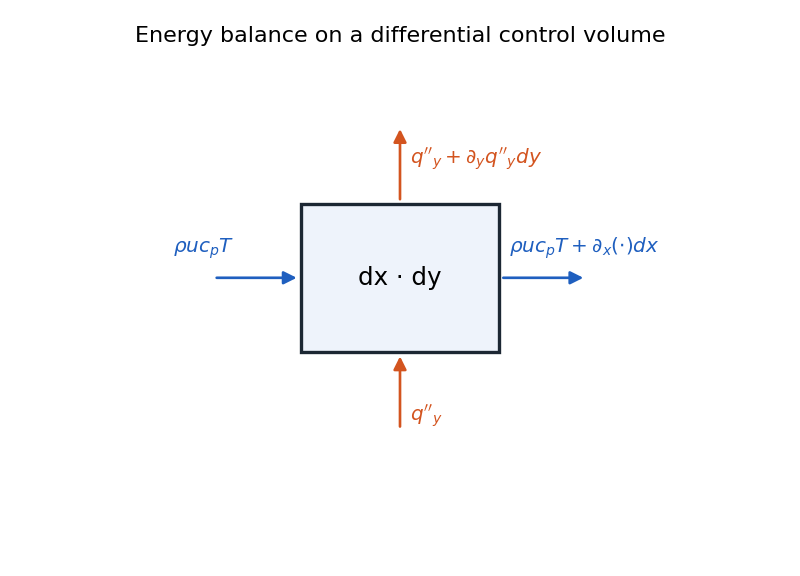
\includegraphics[width=0.75\linewidth]{pics/fig_1.png}
% \end{figure}
% %
% \paragraph{Energy In and Out in the \(x\)-Direction:}
% At the left face (at \(x\)), the total energy flux (per unit time) is given by
% \[
%     \left\{\text{advection } + \text{conduction}\right\}\Bigl\vert_{x} = \left[\rho c_p u\,T + q_x^{\prime\prime}\right]_{x} \; 1\cdot dy,
% \]
% and at the right face (at \(x+dx\)) it is
% \[
%     \left\{\text{advection } + \text{conduction}\right\}\Bigl\vert_{x+dx} = \left[\rho c_p u\,T + q_x^{\prime\prime}\right]_{x+dx} \; 1\cdot dy.
% \]
% Using a Taylor series expansion for a small \(dx\), we have
% \[
% \rho c_p (uT) \big|_{x+dx} \approx \rho c_p uT + \frac{\partial}{\partial x}(\rho c_p uT)\,1\cdot dx,
% \]
% \[
% q_x^{\prime\prime}\big|_{x+dx} \approx q_x^{\prime\prime} + \frac{\partial q_x^{\prime\prime}}{\partial x}\,1\cdot dx.
% \]
% Thus, the net energy flux (energy out minus in) along the \(x\)-direction is
% \[
% \Delta E_x = -\left[\frac{\partial}{\partial x}(\rho c_p uT) + \frac{\partial q_x^{\prime\prime}}{\partial x}\right]dx\,dy.
% \]

% \paragraph{Energy In and Out in the \(y\)-Direction:}
% Similarly, along the \(y\)-direction the net energy flux is
% \[
% \Delta E_y = -\left[\frac{\partial}{\partial y}(\rho c_p vT) + \frac{\partial q_y^{\prime\prime}}{\partial y}\right]dx\,dy.
% \]
% %
% \paragraph{Energy Generation:}
% Let \(S\) be the volumetric rate of energy generation (per unit volume). Then the energy generated within the control volume is
% %
% \[
%     \dot{E}_{\text{gen}} = S\,dx\,dy.
% \]
% %
% \paragraph{Energy Balance:}
% For steady state (no energy accumulation) the net energy change must equal the energy generated:
% \[
%     \sum E_{in} - \sum E_{out} + \dot{E}_{\text{gen}} = 0 \Rightarrow
%     \Delta E_x + \Delta E_y + \dot{E}_{\text{gen}} = 0.
% \]
% Substituting the expressions above, we obtain
% \[
%     -\left[\frac{\partial}{\partial x}(\rho c_p uT) + \frac{\partial q_x^{\prime\prime}}{\partial x} + \frac{\partial}{\partial y}(\rho c_p vT) + \frac{\partial q_y^{\prime\prime}}{\partial y}\right]dx\,dy + S\,dx\,dy = 0.
% \]
% Dividing through by \(dx\,dy\) gives
% \[
%     \frac{\partial}{\partial x}(\rho c_p uT) + \frac{\partial}{\partial y}(\rho c_p vT) + \frac{\partial q_x^{\prime\prime}}{\partial x} + \frac{\partial q_y^{\prime\prime}}{\partial y} = S.
% \]

% \paragraph{Substituting Fourier's Law:}
% Since the conductive heat flux is given by
% \[
% q_x^{\prime\prime} = -k\,\frac{\partial T}{\partial x} \quad \text{and} \quad q_y^{\prime\prime} = -k\,\frac{\partial T}{\partial y},
% \]
% we have
% \[
% \frac{\partial q_x^{\prime\prime}}{\partial x} = -\frac{\partial}{\partial x}\left(k\,\frac{\partial T}{\partial x}\right), \quad \frac{\partial q_y^{\prime\prime}}{\partial y} = -\frac{\partial}{\partial y}\left(k\,\frac{\partial T}{\partial y}\right).
% \]
% Substitute these into the energy balance:
% \[
%     \frac{\partial}{\partial x}(\rho c_p uT) + \frac{\partial}{\partial y}(\rho c_p vT) - \frac{\partial}{\partial x}\left(k\,\frac{\partial T}{\partial x}\right) - \frac{\partial}{\partial y}\left(k\,\frac{\partial T}{\partial y}\right) = S.
% \]

% \paragraph{Simplification:}
% For constant properties (\(\rho\), \(c_p\), and \(k\)) the convection terms can be expressed as
% \[
%     \rho c_p\left(u\,\frac{\partial T}{\partial x} + v\,\frac{\partial T}{\partial y}\right),
% \]
% and the conduction terms become
% \[
%     k\left(\frac{\partial^2 T}{\partial x^2} + \frac{\partial^2 T}{\partial y^2}\right).
% \]
% Thus, the energy equation simplifies to
% \[
%     \rho c_p\left(u\,\frac{\partial T}{\partial x} + v\,\frac{\partial T}{\partial y}\right) = k\left(\frac{\partial^2 T}{\partial x^2} + \frac{\partial^2 T}{\partial y^2}\right) + S.
% \]
% Dividing by \(\rho c_p\) yields the final form:
% \[
% u\,\frac{\partial T}{\partial x} + v\,\frac{\partial T}{\partial y} = \frac{k}{\rho c_p}\left(\frac{\partial^2 T}{\partial x^2} + \frac{\partial^2 T}{\partial y^2}\right) + \frac{S}{\rho c_p}.
% \]
% This is the complete energy equation for convection (advection) with conduction and internal energy generation in a two-dimensional steady-state flow.
% %
% \paragraph{Key Takeaways:}
% \begin{itemize}
%     \item The energy equation accounts for conduction (via Fourier's law), advection (through the term \(\rho c_p u\,T\), representing the energy carried by the moving fluid), and internal heat sources (\(S\)).
%     \item In a bulk energy balance for a control volume, \(\rho c_p u\,T\) quantifies the energy transport due to the fluid's motion, whereas at a surface the convective heat transfer is modeled by Newton's law of cooling, \(hA(T_s-T_\infty)\), which involves the temperature difference between the surface and the ambient.
%     \item When coupled with the momentum and continuity equations, the energy equation provides a complete framework for solving convection problems.
%     \item The heat diffusion equation is a special case of the energy equation when advection is neglected (i.e., when velocity is zero).
%     \item Numerical solvers typically treat conduction as a subset of the general energy equation.
% \end{itemize}


%%%%%%%%%%%%%%%%%%%%%%%%%%%%%%%%%%%%%%%%%%%%%%%%%%%%
\section*{Energy Equation for Convection}
\addcontentsline{toc}{section}{Energy Equation for Convection}
\label{subsec:energy_viscous}
%%%%%%%%%%%%%%%%%%%%%%%%%%%%%%%%%%%%%%%%%%%%%%%%%%%%

Consider a two-dimensional differential control volume of size \(dx \times dy\) and unit depth.  
Energy enters and leaves through both conduction and convection.  
The advective term \(\rho c_p u\,T\) accounts for energy carried by the bulk flow, whereas conduction is governed by Fourier’s law.  
(At boundaries, one often expresses convection with Newton’s law of cooling, \(hA\!\left(T_s - T_\infty\right)\), which involves the surface–ambient temperature difference.)
%
\begin{figure}[H]
    \centering
    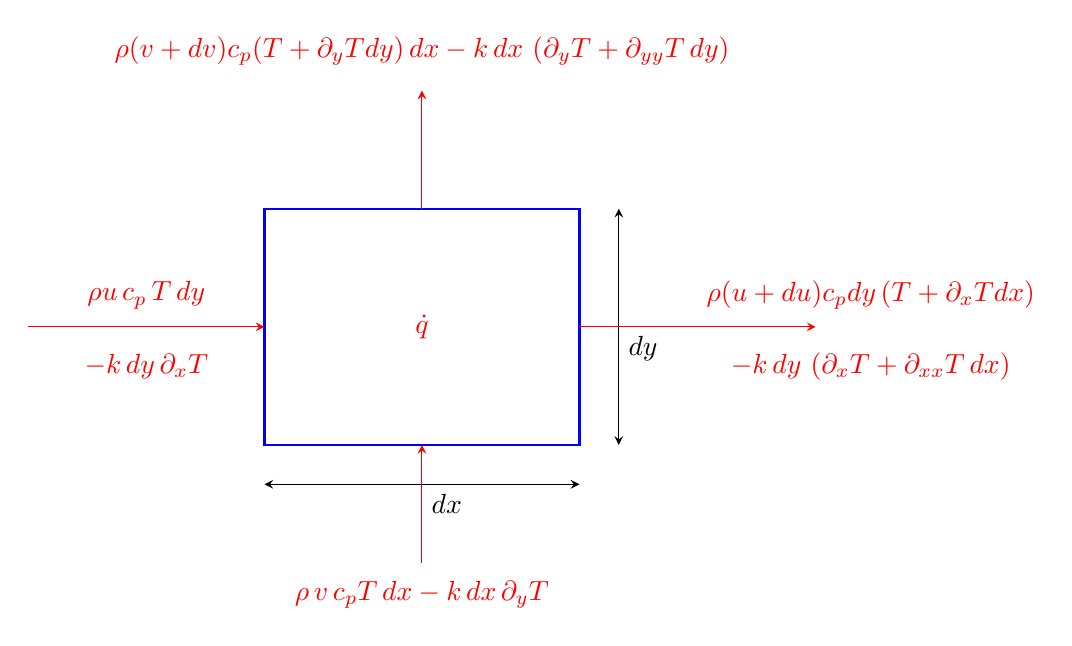
\begin{tikzpicture}[>=stealth]
    % Define convenient lengths for dx and dy
    \def\dx{4}
    \def\dy{3}
    
    % Draw the control-volume rectangle
    \draw[thick, blue] (0,0) rectangle (\dx,\dy);
    
    % Label dx and dy
    \draw[<->] (0,-0.5) -- (\dx,-0.5) node[midway,below right] {$dx$};
    \draw[<->] (\dx+0.5,0) -- (\dx+0.5,\dy) node[midway,below right] {$dy$};
    
    % Left edge - energy in
    \draw[red, ->] (-3,\dy/2) -- (0,\dy/2);
    \node[red, align=left] at (-1.5,\dy/2+0.4) {$\rho u\,c_p\,T\,dy $};
    \node[red, align=left] at (-1.5,\dy/2-0.5) {$-k\,dy \, \partial_x T$};
    
    % Right edge - energy out
    \draw[red, ->] (\dx,\dy/2) -- (\dx+3,\dy/2);
    \node[red, align=left] at (\dx+3.7,\dy/2+0.4) {$\rho(u + du)c_p dy \left(T + \partial_x T dx\right) $};
    \node[red, align=left] at (\dx+3.7,\dy/2-0.5) {$-k\,dy\, \left(\partial_x T + \partial_{xx} T \,dx\right)$};
    
    % Bottom edge - energy in
    \draw[red, ->] (\dx/2,-1.5) -- (\dx/2,0);
    \node[red, align=center] at (\dx/2,-1.9) {$\rho\, v\,c_p T\,dx - k\,dx \,\partial_y T$};
    
    % Top edge - energy out
    \draw[red, ->] (\dx/2,\dy) -- (\dx/2,\dy+1.5);
    \node[red, align=center] at (\dx/2,\dy+2.0) {$\rho(v + dv)c_p(T + \partial_y T dy)\,dx -k\,dx\, \left(\partial_y T + \partial_{yy} T \,dy \right)$};
    
    % Heat generation in the center
    \node[red] at (\dx/2,\dy/2) {$\dot{q}$};
    
\end{tikzpicture}
    % \caption{Schematic of the differential control volume showing conduction and convection terms.}
\end{figure}
%
\paragraph{Assumptions:}
\begin{itemize}
    \item steady state: $\partial_0 T = 0$
    \item constant properties 
    \item isotropic $k$
    \item no radiation
\end{itemize}
%
%
\paragraph{Differential energy balance.}
\[
    \begin{aligned}
    &
    \dot{\mathrm{E}}_{\text {in }}-\dot{\mathrm{E}}_{\text {out }}+\dot{\mathrm{E}}_{\text {gen }}=0
    \\[0.5em]
    &-\Bigl[
      \rho u c_p \,\partial_x T \,dx\,dy
      + \rho\,\mathrm{d}u\,c_p\,T\,dy
      + \rho v c_p \,\partial_y T \,dx\,dy
      + \rho\,\mathrm{d}v\,c_p\,T\,dx
    \Bigr]
    \\[0.3em]
    &\quad
    + k \,\partial_{xx} T \,dx\,dy
    + k \,\partial_{yy} T \,dx\,dy  
    \\[0.3em]
    &\quad
    -\Bigl[
      \rho\,\mathrm{d}u\,c_p\,\partial_x T \,dy\,dx
      + \rho\,\mathrm{d}v\,c_p\,\partial_y T \,dy\,dx
    \Bigr]
    + \dot{q}\,dx\,dy
    =0 
    \end{aligned}
\]
%
\paragraph{Viscous dissipation:}
Viscous effects convert mechanical energy into heat. In 2D, the dissipation term is expressed as ($\mathrm{W/m^3}$)
%
\[
\mu\Phi
= \mu\!\left[
  2\!\left(\partial_x u\right)^{2}
  + 2\!\left(\partial_y v\right)^{2}
  + \left(\partial_y u + \partial_x v\right)^{2}
\right]
\]

Adding this term to the balance yields
\[
    \begin{aligned}
    &-\Bigl[
      \rho u c_p \,\partial_x T \,dx\,dy
      + \rho\,\mathrm{d}u\,c_p\,T\,dy
      + \rho v c_p \,\partial_y T \,dx\,dy
      + \rho\,\mathrm{d}v\,c_p\,T\,dx
    \Bigr] 
    \\[0.3em]
    &\quad
    + k \,\partial_{xx} T \,dx\,dy
    + k \,\partial_{yy} T \,dx\,dy
    -\Bigl[
      \rho\,\mathrm{d}u\,c_p\,\partial_x T \,dy\,dx
      + \rho\,\mathrm{d}v\,c_p\,\partial_y T \,dy\,dx
    \Bigr] \\[0.3em]
    &\quad
    + \dot{q}\,dx\,dy
    + \mu\Phi\,dx\,dy
    =0 
    \end{aligned}
\]
%
Terms such as \(\mathrm{d}u\,dy\,dx\) and \(\mathrm{d}v\,dy\,dx\) are negligibly small.  
After division by \(dx\,dy\),
\[
\begin{aligned}
    &-\rho u c_p \partial_x T
    -\rho c_p T\,\partial_x u
    -\rho v c_p \partial_y T
    -\rho c_p T\,\partial_y v
    +k\partial_{xx} T
    +k\partial_{yy} T
    +\dot{q}
    +\mu\Phi
    =0
    \\[1em]
    &-\rho u c_p \partial_x T
    -\rho c_p T (\,\partial_x u + \,\partial_y v)
    -\rho v c_p \partial_y T
    +k\partial_{xx} T
    +k\partial_{yy} T
    +\dot{q}
    +\mu\Phi
    =0
\end{aligned}
\]
%
From continuity, we have
\[
    \partial_x u + \,\partial_y v = 0
\]
Therefore,
\[
    \begin{aligned}
    &    \rho u c_p \partial_x T
    + \rho v c_p \partial_y T
    = k\left(\partial_{xx} T + \partial_{yy} T\right)
    + \dot{q}
    + \mu\Phi
    \\[1em]
    & \boxed{\rho c_p 
    (u\,\partial_x T
    + v\,\partial_y T)
    = k\left(\partial_{xx} T + \partial_{yy} T\right)
    + \dot{q}
    + \mu\Phi
    }
    \end{aligned}
\]
This form clearly shows the contributions of conduction, convection, internal heat generation, and viscous dissipation.

% %%%%%%%%%%%%%%%%%%%%%%%%%%%%%%%%%%%%%%%%%%%%%%%%%%%%
% \subsubsection*{Energy Equation for Convection}
% \addcontentsline{toc}{subsubsection}{Energy Equation for Convection}
% %%%%%%%%%%%%%%%%%%%%%%%%%%%%%%%%%%%%%%%%%%%%%%%%%%%%
% Consider a differential control volume with dimensions \(dx\) and \(dy\) (unit depth). The energy entering and leaving the control volume includes contributions from conduction and convection. Note that the convection (or advection) term, \(\rho c_p u\,T\), represents the energy carried by the fluid due to its bulk motion, while the conduction term is modeled via Fourier’s law. In contrast, when applying boundary conditions, convective heat transfer is often expressed using Newton's law of cooling, \(hA(T_s-T_\infty)\), which involves the temperature difference between the surface and the ambient.

% %
% \begin{figure}[H]
%     \centering
%     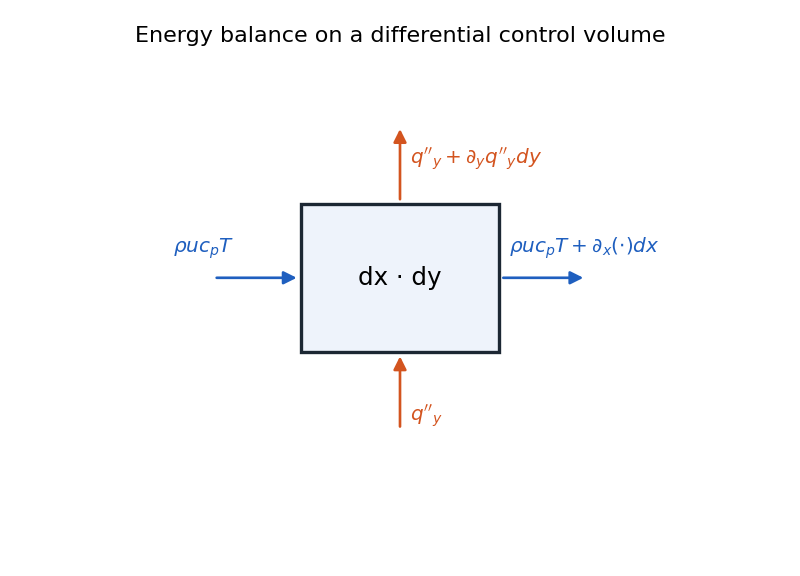
\includegraphics[width=0.75\linewidth]{pics/fig_1.png}
% \end{figure}
% %
% \paragraph{Energy In and Out in the \(x\)-Direction:}
% At the left face (at \(x\)), the total energy flux (per unit time) is given by
% \[
%     \left\{\text{advection } + \text{conduction}\right\}\Bigl\vert_{x} = \left[\rho c_p u\,T + q_x^{\prime\prime}\right]_{x} \; 1\cdot dy,
% \]
% and at the right face (at \(x+dx\)) it is
% \[
%     \left\{\text{advection } + \text{conduction}\right\}\Bigl\vert_{x+dx} = \left[\rho c_p u\,T + q_x^{\prime\prime}\right]_{x+dx} \; 1\cdot dy.
% \]
% Using a Taylor series expansion for a small \(dx\), we have
% \[
% \rho c_p (uT) \big|_{x+dx} \approx \rho c_p uT + \frac{\partial}{\partial x}(\rho c_p uT)\,1\cdot dx,
% \]
% \[
% q_x^{\prime\prime}\big|_{x+dx} \approx q_x^{\prime\prime} + \frac{\partial q_x^{\prime\prime}}{\partial x}\,1\cdot dx.
% \]
% Thus, the net energy flux (energy out minus in) along the \(x\)-direction is
% \[
% \Delta E_x = -\left[\frac{\partial}{\partial x}(\rho c_p uT) + \frac{\partial q_x^{\prime\prime}}{\partial x}\right]dx\,dy.
% \]

% \paragraph{Energy In and Out in the \(y\)-Direction:}
% Similarly, along the \(y\)-direction the net energy flux is
% \[
% \Delta E_y = -\left[\frac{\partial}{\partial y}(\rho c_p vT) + \frac{\partial q_y^{\prime\prime}}{\partial y}\right]dx\,dy.
% \]
% %
% \paragraph{Additional Energy Contributions:}
% In many practical problems, additional energy sources must be included:
% \begin{enumerate}
%     \item \textbf{Internal Heat Generation:} Let \(\dot{q}\) be the volumetric rate of energy generation (e.g., chemical reactions or radiation absorption). Then the energy added per unit time is
%     \[
%         \dot{E}_{\text{gen}} = \dot{q}\,dx\,dy
%     \]
%     \item \textbf{Viscous Dissipation:} 
%     \begin{definition}
%     Viscous effects convert mechanical energy into heat. In two dimensions, the dissipation term is expressed as
%     \[
%         \mu\Phi = \mu\left\{2\left[\left(\frac{\partial u}{\partial x}\right)^2 + \left(\frac{\partial v}{\partial y}\right)^2\right] + \left(\frac{\partial u}{\partial y} + \frac{\partial v}{\partial x}\right)^2\right\}
%     \]
%     \end{definition}

%     This term represents the rate of energy conversion per unit volume due to internal friction.
% \end{enumerate}

% \paragraph{Energy Balance:}
% For steady state (no energy accumulation), the net energy change must equal the energy added by internal sources and viscous dissipation:
% \[
%     \Delta E_x + \Delta E_y + \dot{E}_{\text{gen}} + (\mu\Phi\,dx\,dy) = 0.
% \]
% Substituting the expressions above, we obtain
% \[
% -\left[\frac{\partial}{\partial x}(\rho c_p uT) + \frac{\partial q_x^{\prime\prime}}{\partial x} + \frac{\partial}{\partial y}(\rho c_p vT) + \frac{\partial q_y^{\prime\prime}}{\partial y}\right]dx\,dy + \left(\dot{q} + \mu\Phi\right)dx\,dy = 0.
% \]
% Dividing through by \(dx\,dy\) gives
% \[
% \frac{\partial}{\partial x}(\rho c_p uT) + \frac{\partial}{\partial y}(\rho c_p vT) + \frac{\partial q_x^{\prime\prime}}{\partial x} + \frac{\partial q_y^{\prime\prime}}{\partial y} = \dot{q} + \mu\Phi.
% \]

% \paragraph{Substituting Fourier's Law:}
% Since the conductive heat flux is given by
% \[
% q_x^{\prime\prime} = -k\,\frac{\partial T}{\partial x} \quad \text{and} \quad q_y^{\prime\prime} = -k\,\frac{\partial T}{\partial y},
% \]
% we have
% \[
% \frac{\partial q_x^{\prime\prime}}{\partial x} = -\frac{\partial}{\partial x}\left(k\,\frac{\partial T}{\partial x}\right), \quad \frac{\partial q_y^{\prime\prime}}{\partial y} = -\frac{\partial}{\partial y}\left(k\,\frac{\partial T}{\partial y}\right).
% \]
% Substituting these into the energy balance yields:
% \[
% \frac{\partial}{\partial x}(\rho c_p uT) + \frac{\partial}{\partial y}(\rho c_p vT) - \frac{\partial}{\partial x}\left(k\,\frac{\partial T}{\partial x}\right) - \frac{\partial}{\partial y}\left(k\,\frac{\partial T}{\partial y}\right) = \dot{q} + \mu\Phi.
% \]

% \paragraph{Simplification:}
% For constant properties (\(\rho\), \(c_p\), and \(k\)), the convection terms become
% \[
%     \rho c_p\left(u\,\frac{\partial T}{\partial x} + v\,\frac{\partial T}{\partial y}\right)
% \]
% and the conduction terms simplify to
% \[
%     k\left(\frac{\partial^2 T}{\partial x^2} + \frac{\partial^2 T}{\partial y^2}\right)
% \]
% \begin{definition}
% Thus, the steady-state energy equation is:
% \[
%     \rho c_p\left(u\,\frac{\partial T}{\partial x} + v\,\frac{\partial T}{\partial y}\right) = k\left(\frac{\partial^2 T}{\partial x^2} + \frac{\partial^2 T}{\partial y^2}\right) + \dot{q} + \mu\Phi.
% \]
% or
% \[
%     \rho c_p \left(u\frac{\partial T}{\partial x} + v\frac{\partial T}{\partial y}\right) = k\nabla^2 T + \dot{q} + \mu\Phi
% \]
% \end{definition}
% %
% 
